\documentclass[conference]{IEEEtran}
\usepackage[utf8]{inputenc}
\usepackage{amsmath,amssymb,amsfonts}
\usepackage{newtxtext,newtxmath}
\usepackage{graphicx}
\usepackage{booktabs}
\usepackage{tabularx}
\usepackage{stfloats}
\usepackage{array}
\usepackage{makecell}
\usepackage{xcolor}
\definecolor{citeblue}{RGB}{0, 102, 204}
\usepackage[colorlinks=true, citecolor=citeblue, linkcolor=black, urlcolor=citeblue]{hyperref}
\usepackage{cite}
\usepackage{microtype}
\usepackage[font=footnotesize,labelfont=bf,labelsep=period]{caption}
\usepackage{tcolorbox}

% Float parameters to allow 2 double floats per page
\setcounter{topnumber}{3}
\setcounter{bottomnumber}{3}
\setcounter{totalnumber}{6}
\setcounter{dbltopnumber}{2}
\renewcommand{\topfraction}{0.98}
\renewcommand{\bottomfraction}{0.98}
\renewcommand{\textfraction}{0.02}
\renewcommand{\floatpagefraction}{0.75}
\renewcommand{\dbltopfraction}{0.98}
\renewcommand{\dblfloatpagefraction}{0.75}

% Display math and float spacing
\setlength{\textfloatsep}{6pt plus 1pt minus 1pt}
\setlength{\dbltextfloatsep}{6pt plus 1pt minus 1pt}
\setlength{\floatsep}{5pt plus 1pt minus 1pt}
\setlength{\dblfloatsep}{5pt plus 1pt minus 1pt}
\setlength{\intextsep}{5pt plus 1pt minus 1pt}
\setlength{\abovedisplayskip}{4pt plus 1pt minus 1pt}
\setlength{\belowdisplayskip}{4pt plus 1pt minus 1pt}
\setlength{\abovedisplayshortskip}{2pt plus 1pt}
\setlength{\belowdisplayshortskip}{2pt plus 1pt}

% Strict font size hierarchy:
% size đề mục (\large\bfseries ~12pt / \normalsize\bfseries 10pt) > size nội dung (10pt) > size bảng (\footnotesize 8pt)
\makeatletter
\renewcommand\section{\@startsection{section}{1}{\z@}{1.1ex plus 0.2ex minus 0.1ex}{0.5ex plus 0.1ex}{\large\bfseries}}
\renewcommand\subsection{\@startsection{subsection}{2}{\z@}{0.9ex plus 0.2ex minus 0.1ex}{0.4ex plus 0.1ex}{\normalsize\bfseries}}
\renewcommand\subsubsection{\@startsection{subsubsection}{3}{\z@}{0.8ex plus 0.1ex minus 0.1ex}{0.3ex plus 0.1ex}{\normalsize\itshape}}
\makeatother

% Abstract & Keywords formatting: bold label only, regular content
\renewenvironment{abstract}{%
  \normalfont\small
  \textbf{Abstract}---%
  \mdseries
}{%
  \par\vspace{4pt}
}

\renewenvironment{IEEEkeywords}{%
  \normalfont\small
  \textbf{Index Terms}---%
  \mdseries
}{%
  \par\vspace{6pt}
}

\pagestyle{plain}
\begin{document}

\title{\Large\bfseries GEMMA-CLIP: Fine-Grained Pet Breed Classification with Morphological Knowledge, Prompt Optimization and Multi-View Inference}

\author{
\IEEEauthorblockN{Nguyen Huu Hoang Luan, Ton That Van}
\IEEEauthorblockA{Department of Information Technology, University of Science and Technology -- The University of Danang\\
Email: \{102230028; 102230055\}@sv1.dut.udn.vn\ \ GitHub: \url{https://github.com/LuanNguyen23T/CLIP-Animal-Classifier}}
}

\maketitle
\thispagestyle{plain}

\begin{abstract}
We study parameter-efficient adaptation of a frozen CLIP ViT-B/32 model using morphological descriptors generated locally by Gemma~4 E4B. The framework separates an inspectable concept-score branch, a fixed morphological centroid bank, compact-trait prompt tuning, and a residual visual adapter. On the official Oxford-IIIT Pet test set (3,669 images), Gemma-DualStream combines prompt tuning with fixed centroids and reaches 92.07\% Top-1 under 5-View TTA using 2,048 trainable prompt parameters. Its 0.68-point margin over standard CoOp is not significant in the reported paired McNemar test ($p=0.0696$). In the separate three-seed few-shot benchmark at $K=1$, DualStream has lower observed variation than CoOp (87.55 $\pm$ 0.28\% versus 86.32 $\pm$ 2.25\%); this descriptive result is limited to the tested seeds. On the official Stanford Dogs split (12,000 train / 8,580 test), Gemma-CoOp obtains 64.45\%, DualStream 64.17\%, and standard CoOp 63.62\% using single-view cached features. Concept scores can be inspected by anatomical group, but their causal faithfulness has not been established. The 2,048-parameter count excludes frozen CLIP weights, offline descriptor generation, and inference cost. Our contribution is the controlled study of trainable-parameter cost, inspectable morphological scores, and behavior under few-shot supervision.
\end{abstract}

\begin{IEEEkeywords}
FGVC, Vision-Language Models (VLM), CLIP, Gemma~4 SLM, CoOp, CBM, TTA.
\end{IEEEkeywords}

\section{Introduction}

FGVC requires vision systems to resolve minute, localized anatomical boundaries amidst large posture and illumination variations~\cite{parkhi2012cats}. In Oxford-IIIT Pet, Ragdoll and Birman cats share pointed cream coats and blue eyes; Birman has a characteristic symmetrical glove and lace pattern, but white feet alone are not a definitive discriminator because mitted Ragdolls can also have them~\cite{cfa_ragdoll, cfa_birman}. Similarly, Staffordshire Bull Terriers and American Pit Bull Terriers share muscular builds, separated primarily by cheekbone width to mandibular taper ratios.

Global visual classifiers frequently fail on such localized cues. Contrastive Language-Image Pre-training (CLIP; Radford et al.~\cite{radford2021learning}) enables zero-shot classification via cosine similarity between visual embedding $f(x)$ and text prompt embedding $w_c$, yet generic prompts (\emph{``a photo of a \{class\}''}) omit diagnostic morphology. While parameter-efficient fine-tuning (PEFT) methods---such as CoOp~\cite{zhou2022learning}, CLIP-Adapter~\cite{gao2024clip}, and Tip-Adapter~\cite{zhang2022tip}---learn continuous prompts or residual bottlenecks, standard continuous prompt vectors lack explicit anatomical grounding, can exhibit sensitivity to sample selection under few-shot initialization ($K=1$, where CoOp averages 86.32\% with high variance across random seeds), and appending lengthy descriptive text risks dispersing self-attention gradients across CLIP layers. Furthermore, prior LLM-guided vision approaches (e.g., CuPL, LaBo) rely on remote proprietary cloud APIs (GPT-3/4), incurring recurring monetary costs, latency overhead, and privacy constraints.

We study how locally generated morphological descriptors can support parameter-efficient fine-grained classification. Gemma-CLIP pairs a frozen CLIP ViT-B/32 backbone with Gemma-generated attributes along five anatomical axes. These feed a 185-concept projection for score inspection, a fixed morphological centroid bank, compact-trait CoOp prompt tuning, and a separately evaluated visual adapter. The Gemma-DualStream configuration fuses CoOp and centroid scores without using the visual adapter; it trains 2,048 prompt parameters. Our evaluation examines (i) accuracy and trainable-parameter cost under explicit data and inference protocols, (ii) concept-score examples and their limitations, and (iii) few-shot behavior over three seeds. On the Oxford-IIIT Pet 9:1 training protocol, DualStream obtains 92.07\% 5-View TTA versus 91.39\% for standard CoOp; the paired comparison does not establish a difference at the 0.05 significance level ($p=0.0696$).

\begin{figure*}[t]
\centering
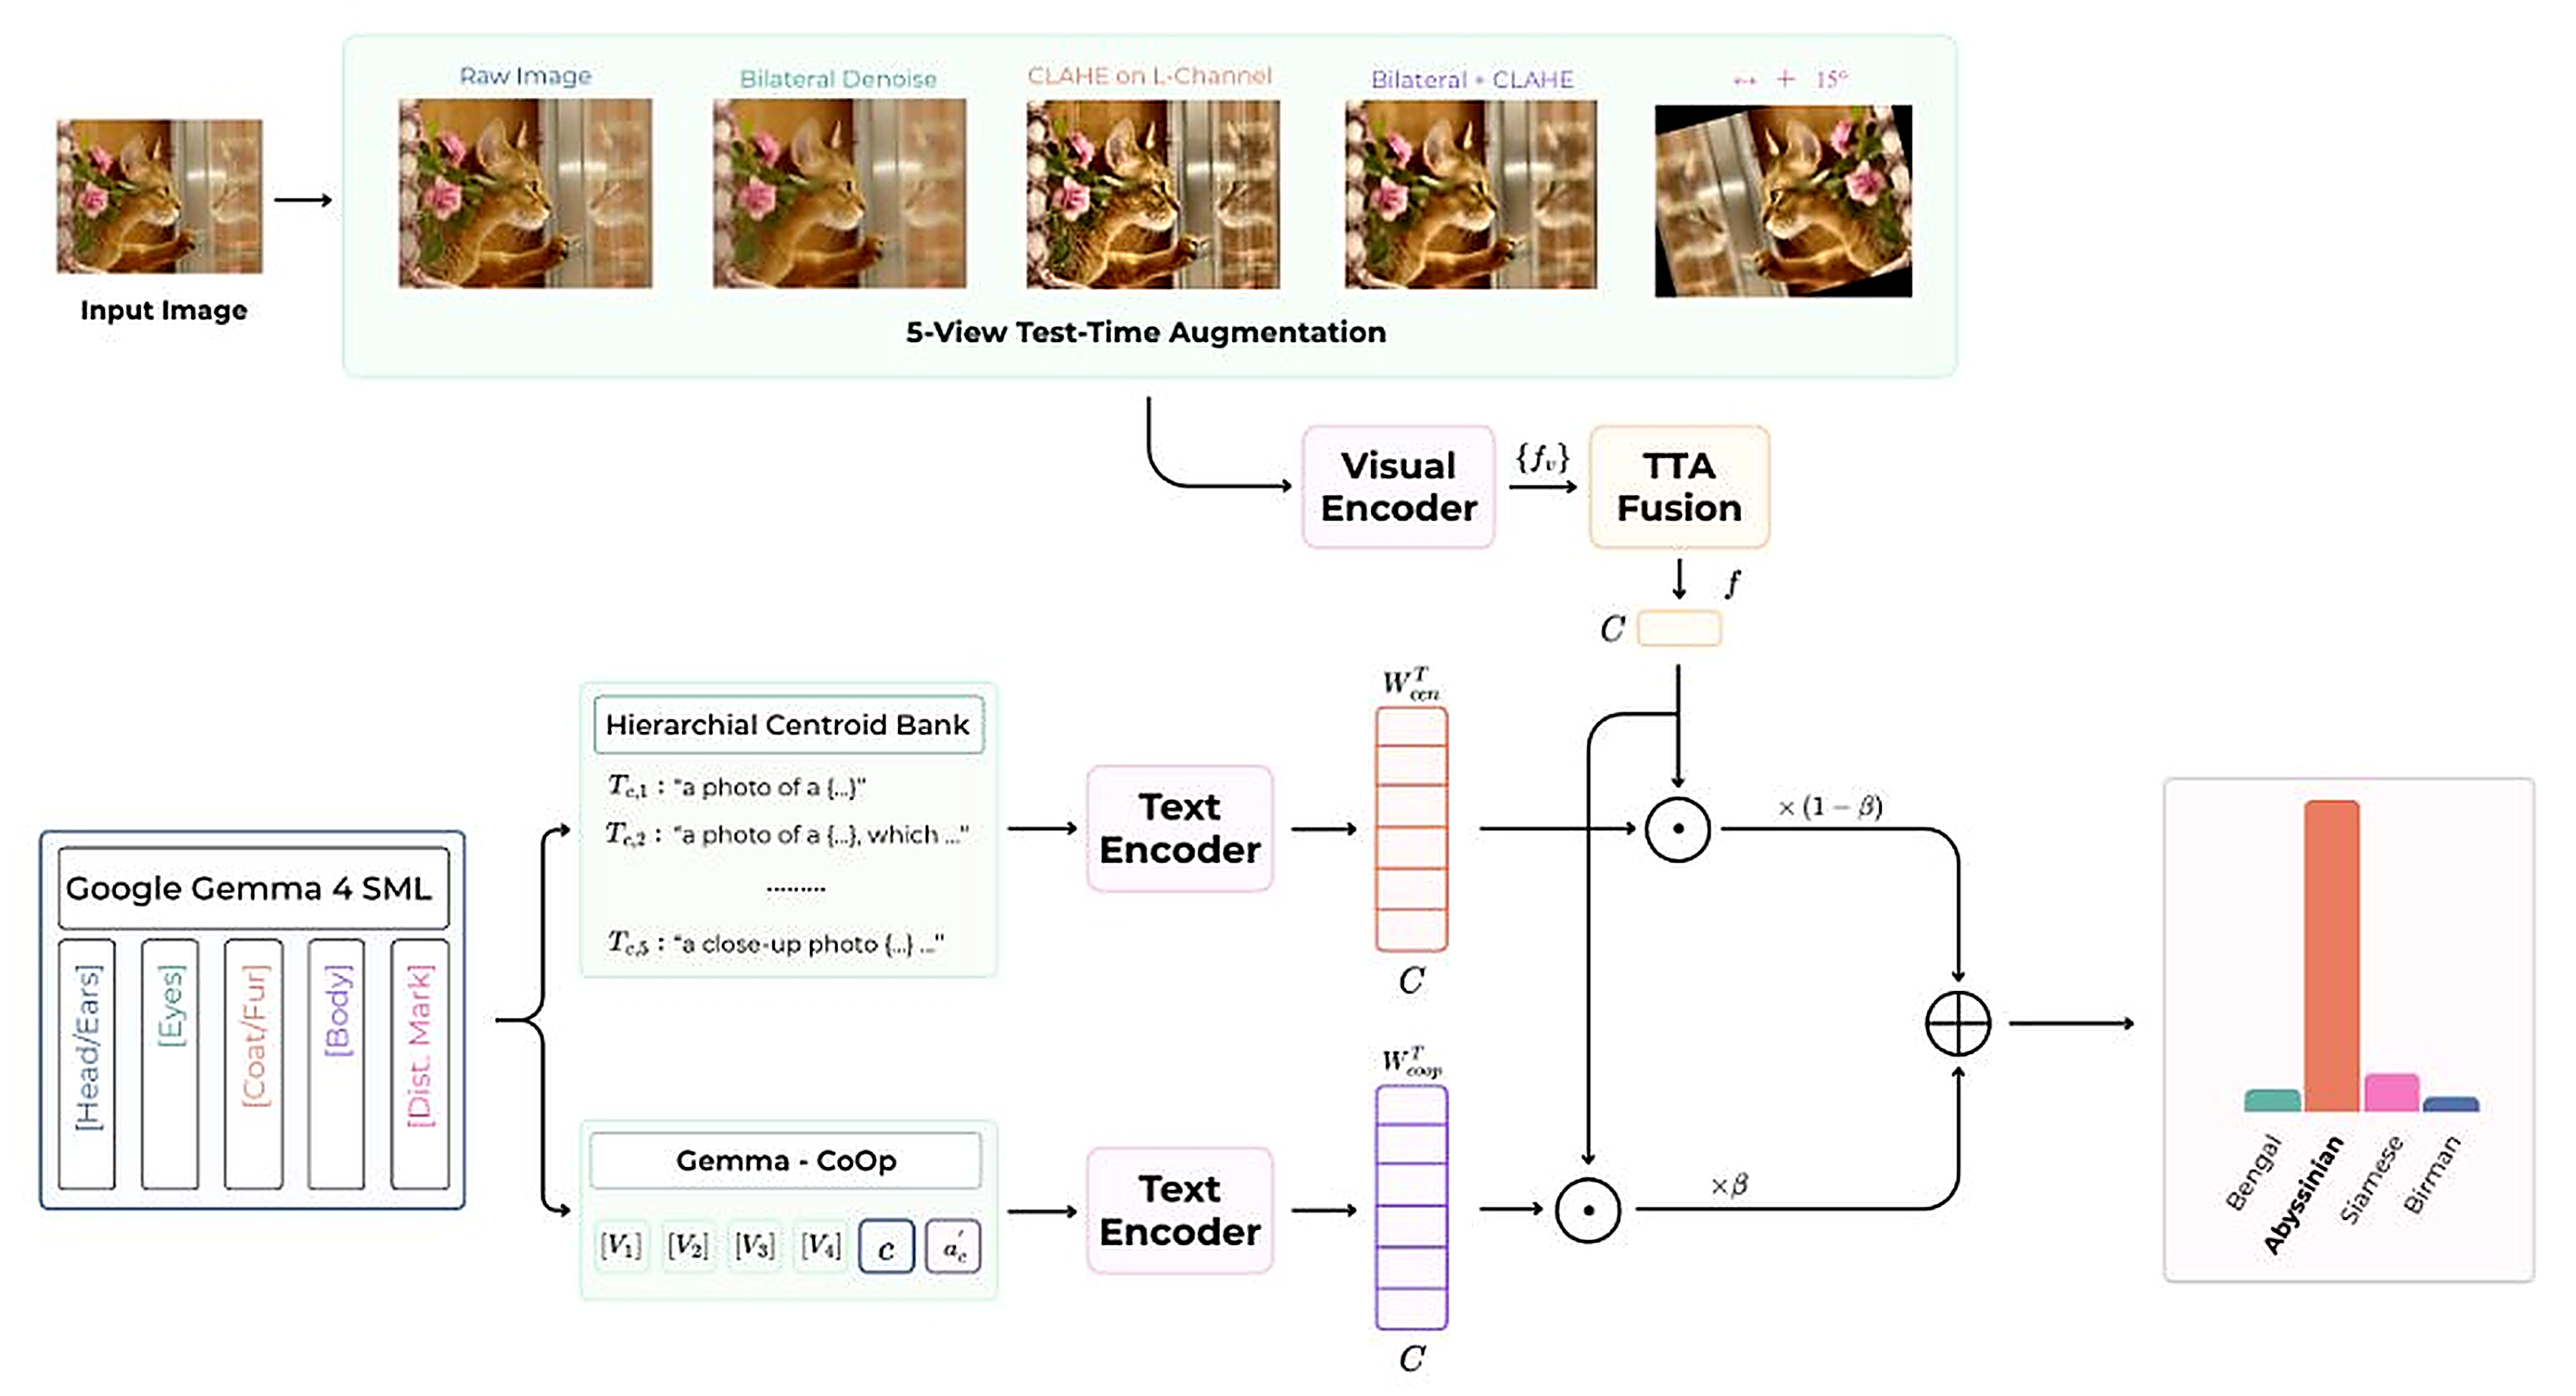
\includegraphics[width=\textwidth]{architecture.png}
\caption{Architecture of Gemma-CLIP: coupling 5-View Test-Time Augmentation (TTA), frozen CLIP visual encoding, non-parametric Hierarchical Centroid Bank distilled from on-device Google Gemma~4 SLM across 5 anatomical axes, and parameterized Gemma-CoOp soft prompt tuning with dual-stream logit fusion. Note: In the parameter-efficient Gemma-DualStream setting (2,048 parameters), the visual adapter is bypassed ($f'(x) \equiv f(x)$), directly combining Gemma-CoOp soft prompt tuning with the centroid bank.}
\label{fig:arch}
\end{figure*}

\section{Related Work \& Baseline Definitions}

\subsection{Vision-Language Models (CLIP)}
CLIP~\cite{radford2021learning} maps visual $f(x)$ and text $w_c$ embeddings into a shared normalized space $\mathbb{R}^D$ ($D=512$). Class probabilities are given by:
\begin{equation}
P(y = c \mid x) = \frac{\exp(\tau \langle f(x), w_c \rangle)}{\sum_{j=1}^C \exp(\tau \langle f(x), w_j \rangle)}
\end{equation}
where $f(x) \in \mathbb{R}^{512}$ denotes the $L_2$-normalized visual feature vector extracted by the frozen Vision Transformer ($\|f(x)\|_2 = 1$), $w_c \in \mathbb{R}^{512}$ is the normalized text embedding of class $c$ ($\|w_c\|_2 = 1$), $\tau$ represents the learned logit scale parameter ($\tau \approx 100.0$ at evaluation), and $C$ is the total number of candidate classes ($C=37$ for Oxford-IIIT Pet and $C=120$ for Stanford Dogs). Evaluated on Oxford-IIIT Pet, raw class names achieve 80.16\% (80.68\% TTA), while handcrafted prompts achieve 87.49\% (87.98\% TTA).

\subsection{PEFT Baselines}
CoOp~\cite{zhou2022learning} models prompts as $M$ learnable continuous tokens $[V]_1, \dots, [V]_M \in \mathbb{R}^d$ prepended to fixed class embeddings: $t_c = [[V]_1, \dots, [V]_M, e_c]$ ($M=4, d=512$, 2,048 parameters). CLIP-Adapter~\cite{gao2024clip} inserts a two-layer bottleneck MLP on image features, while Tip-Adapter~\cite{zhang2022tip} builds a non-parametric key-value cache fine-tuned in Tip-Adapter-F.

\subsection{Supervised Upper-Bound References (Ceiling Baselines)}
Supervised models---such as ResNet-50 Cosine Head~\cite{gidaris2018dynamic} (75,815 parameters) and ResNet-50 Prototype~\cite{snell2017prototypical}---train directly on 100\% of labeled training data (3,680 images). While achieving strong full-data accuracy (93.08\%), they require full supervision and suffer pronounced degradation in few-shot regimes ($K=1$: 72.88\%) due to the absence of multimodal foundation priors. We treat them as supervised reference baselines rather than architectural peers.

\subsection{Concept Bottlenecks (CBM) \& LLM Prompting (CuPL, LaBo)}
CBMs~\cite{koh2020concept} route predictions through interpretable concept scores. In parallel, prompt ensembling frameworks query large language models: CuPL~\cite{pratt2023what} queries GPT-3 to generate customized visual descriptive prompts, while LaBo~\cite{yang2023language} constructs concept bottlenecks via submodular selection. In this work, we evaluate official author-released CuPL prompts on Oxford-IIIT Pet alongside locally simulated concept pipelines. Gemma-CLIP departs in three key ways: (i) executes an on-device Gemma~4 SLM locally with zero API cost and full data privacy; (ii) constrains descriptors to AKC/FCI and CFA/TICA standards across 5 canonical anatomical axes; and (iii) anchors PEFT prompt and visual adapter tuning directly to morphological priors.

\begin{table*}[t]
\centering
\caption{Illustrative Gemma-Generated Descriptors for Confusable Breed Pairs; known overgeneralizations are identified rather than treated as diagnostic rules.}
\label{tab:confusable_descriptors}
\vspace{2pt}
\footnotesize
\setlength{\tabcolsep}{5pt}
\renewcommand{\arraystretch}{1.05}
\begin{tabularx}{\textwidth}{p{1.8cm} p{2.2cm} p{6.8cm} X}
\toprule
\textbf{Confusable Pair} & \textbf{Breed \& Registry} & \textbf{Key Anatomical Descriptors (Gemma 4 Distilled)} & \textbf{Key Distinguishing Morphological Feature} \\
\midrule
\textbf{Feline Pair} & \textbf{Birman} \emph{(CFA)} & 
$\bullet$ \texttt{head}: Broad, rounded skull contour.\newline
$\bullet$ \texttt{eyes}: Round, deep sapphire-blue.\newline
$\bullet$ \texttt{coat}: Silky semi-longhair, no undercoat. & 
\textbf{Pure white symmetrical ``gloves''} on all four paws. \\
\cmidrule{2-4}
& \textbf{Ragdoll} \emph{(CFA)} & 
$\bullet$ \texttt{head}: Broad modified wedge, flat plane.\newline
$\bullet$ \texttt{eyes}: Large, vivid blue, oval.\newline
$\bullet$ \texttt{coat}: Semi-long plush, dense undercoat. & 
\textbf{Known descriptor limitation:} the archived Gemma attribute says ``absence of white gloves'', but mitted Ragdolls can have white feet~\cite{cfa_ragdoll}. \\
\midrule
\textbf{Canine Pair} & \textbf{Staffordshire Bull Terrier} \emph{(AKC)} & 
$\bullet$ \texttt{head}: Broad skull; semi-pricked close ears.\newline
$\bullet$ \texttt{body}: Compact, low-slung, short tail.\newline
$\bullet$ \texttt{coat}: Short, dense, sleek double coat. & 
\textbf{Blocky, low-slung silhouette} with extreme muscle density. \\
\cmidrule{2-4}
& \textbf{American Pit Bull Terrier} \emph{(UKC)} & 
$\bullet$ \texttt{head}: Broad skull; semi-erect high-set ears.\newline
$\bullet$ \texttt{body}: Leggier frame, pronounced chest depth.\newline
$\bullet$ \texttt{coat}: Extremely short, smooth single coat. & 
\textbf{Athletic, leggy taper} with pronounced chest depth. \\
\bottomrule
\end{tabularx}
\end{table*}

\section{Proposed Methodology}

\subsection{Local Morphological Knowledge Distillation via Gemma~4 SLM}
Gemma~4 E4B (\texttt{google/gemma-4-e4b})~\cite{gemma2026report} is served locally via LM Studio with deterministic greedy decoding (\texttt{temp=0.0}, \texttt{seed=42}). For each class $c$, the SLM generates structured descriptors across five anatomical axes: \texttt{head\_and\_ears}, \texttt{eyes}, \texttt{coat}, \texttt{body}, and \texttt{distinguishing\_mark} (Appendix~A). Non-visual descriptors are excluded. An existing internal spot-check of 19/185 descriptors reports 18/19 matches to referenced breed-standard descriptions (Appendix~A); this is neither an independent expert review nor validation of the entire attribute bank. We identify a Ragdoll paw-marking overgeneralization below and do not perform an additional audit for this revision. The complete knowledge base is serialized openly in structured JSON format (see Appendix~A for prompt templates and public knowledge base links).

\subsection{185-Dimensional CBM Space \& Morphological Centroids}
Each raw attribute $a_c^{(k)}$ ($k \in \{1..5\}$) is formatted via template $\mathcal{T}_k(\cdot)$ (Appendix~B) and projected through frozen CLIP text encoder $\mathcal{E}_{\text{txt}}$ into normalized vector $w_c^{(k)} \in \mathbb{R}^{512}$.

In the \textbf{Gemma-CBM} stream, stacking all 185 concept vectors forms the morphological concept projection matrix $W_{\text{concept}} \in \mathbb{R}^{185 \times 512}$. For any image embedding $f(x)$, concept activation scores and diagnostic class predictions are computed as:
\begin{equation}
\hat{y}_{\text{CBM}} = \arg\max_{c \in \{1 \dots C\}} \frac{1}{K_{\text{axes}}} \sum_{k=1}^{K_{\text{axes}}} \langle f(x), w_c^{(k)} \rangle
\end{equation}
where $s_{c,k}(x) \in [-1, 1]$ represents the cosine activation score between the normalized image representation $f(x) \in \mathbb{R}^{512}$ and the $k$-th anatomical concept vector $w_c^{(k)} \in \mathbb{R}^{512}$ of class $c$, and $K_{\text{axes}} = 5$ corresponds to the five canonical anatomical axes (\texttt{head\_and\_ears}, \texttt{eyes}, \texttt{coat}, \texttt{body}, \texttt{distinguishing\_mark}). Uniform pooling across these 5 concept scores yields the transparent prediction $\hat{y}_{\text{CBM}}$ across the $C$ candidate categories.

In parallel, the \textbf{Gemma-Centroid} stream constructs an invariant morphological centroid representation for each class $c$ by normalizing the average of its five concept projections:
\begin{equation}
w_c^{\text{centroid}} = \text{Normalize}\left(\frac{1}{5} \sum_{k=1}^5 w_c^{(k)}\right) = \frac{\sum_{k=1}^5 w_c^{(k)}}{\left\|\sum_{k=1}^5 w_c^{(k)}\right\|_2} \in \mathbb{R}^{512}
\end{equation}
where $w_c^{\text{centroid}} \in \mathbb{R}^{512}$ is the $L_2$-normalized mean concept vector for class $c$. Stacking all $C$ centroids forms the static non-parametric text matrix $W_{\text{centroid}} \in \mathbb{R}^{C \times 512}$ ($37 \times 512$ for Pets; $120 \times 512$ for Dogs), serving as fixed semantic anchors for inference and adaptation with zero trainable parameters.

\subsection{Residual Visual Adaptation \& Gemma-CoOp Prompt Optimization}

\subsubsection{Gemma-VisAdapter with Prior Weight Anchoring}
Visual adaptation employs a lightweight two-layer residual bottleneck MLP ($512 \to 64 \to 512$, 65,536 parameters):
\begin{equation}
\Delta f(x) = W_2 \cdot \text{ReLU}(W_1 f(x))
\end{equation}
where $W_1 \in \mathbb{R}^{64 \times 512}$ is a down-projection matrix, $W_2 \in \mathbb{R}^{512 \times 64}$ is an up-projection matrix, and $\text{ReLU}(\cdot) = \max(0, \cdot)$ introduces non-linearity. Zero-initialization ($W_2 \leftarrow 0$) guarantees $\Delta f(x) = 0$ at step 0, strictly preserving pre-trained CLIP representations ($2 \times 512 \times 64 = 65,536$ trainable parameters).

The adapted visual embedding is obtained by residual interpolation:
\begin{equation}
f'(x) = \text{Normalize}\left((1 - \alpha)f(x) + \alpha \cdot \Delta f(x)\right)
\end{equation}
where $\alpha \in [0, 1]$ is the residual blending factor ($\alpha = 0.2$ is our conservative reported operating point), and $f'(x) \in \mathbb{R}^{512}$ is the adapted normalized visual embedding. Classification logits are evaluated against fixed centroid weights via $z_c^{\text{adapter}} = \tau \langle f'(x), w_c^{\text{centroid}} \rangle$.

\begin{table*}[t]
\centering
\caption{Architectural Ablation Performance on Official Test Split (3,669 Images) under Hyperparameter Validation Split (3,310 Train / 370 Val Protocol).}
\label{tab:ablation}
\vspace{2pt}
\footnotesize
\setlength{\tabcolsep}{3.5pt}
\renewcommand{\arraystretch}{1.1}
\begin{tabular*}{\textwidth}{@{\extracolsep{\fill}} p{2.2cm} p{3.6cm} p{3.2cm} >{\centering\arraybackslash}p{1.4cm} >{\centering\arraybackslash}p{1.4cm} >{\centering\arraybackslash}p{1.5cm} >{\centering\arraybackslash}p{1.5cm} >{\centering\arraybackslash}p{1.5cm} @{}}
\toprule
\textbf{Paradigm\newline Category} & \textbf{Evaluated\newline Architecture} & \textbf{Adaptation\newline Mechanism} & \textbf{Trainable\newline Params} & \textbf{Top-1 (\%)\newline Raw} & \textbf{Top-1 (\%)\newline 5-View} & \textbf{Top-5 (\%)\newline 5-View} & \textbf{Macro F1\newline 5-View} \\
\midrule
\textbf{CLIP Baselines} & CLIP Raw Class Names & Zero-Shot Basic & 0 & 80.16\% & 80.68\% & 96.40\% & 77.40\% \\
& CLIP Handcrafted Prompt & Zero-Shot Enriched & 0 & 87.49\% & 87.98\% & 99.21\% & 87.41\% \\
& CLIP 80-Prompt Ensemble & Zero-Shot Multi-Prompt & 0 & 85.20\% & 86.15\% & 97.30\% & 84.56\% \\
& CuPL Official Prompts~\cite{pratt2023what} & LLM-Guided Prompts & 0 & 87.22\% & 87.63\% & 99.62\% & 87.11\% \\
\midrule
\textbf{PEFT Baselines}$^{\dag}$ & Tip-Adapter~\cite{zhang2022tip} & Key-Value Cache & 0 & 87.00\% & 88.06\% & 98.72\% & 87.94\% \\
& Tip-Adapter-F (9:1 Split)~\cite{zhang2022tip} & Tuned Cache & 3,680 & 89.10\% & 89.56\% & 98.96\% & 89.48\% \\
& CLIP-Adapter (9:1 Split)~\cite{gao2024clip} & Visual Residual MLP & 65,536 & 89.42\% & 91.28\% & 99.10\% & 91.22\% \\
& CoOp Baseline (9:1 Split)~\cite{zhou2022learning} & Soft Continuous Tokens & 2,048 & 91.58\% & 91.39\% & 99.70\% & 91.33\% \\
\midrule
\textbf{Supervised Reference} & ResNet-50 Cosine\newline (9:1 Split, Frozen Features) & Normalized Cosine Head\newline (Frozen) & 75,815 & --- & 86.51\% & 99.51\% & 86.31\% \\
& \textbf{ResNet-50 Cosine}\newline \textbf{(Full Ceiling)}$^{\P}$ & Normalized Cosine Head\newline (End-to-End) & 75,815 & \textbf{92.78\%} & \textbf{93.08\%} & \textbf{99.32\%} & \textbf{93.02\%} \\
\midrule
\textbf{Gemma-CLIP (Ours)} & Gemma-CBM$^{\S}$ & 185-Concept Projection & 0 & 81.44\% & 81.52\% & 97.77\% & 79.38\% \\
& Gemma-Centroid & Training-Free Centroid Bank & 0 & 88.14\% & 88.39\% & 99.48\% & 88.11\% \\
& Gemma-ZeroShot & Prompt + Centroid Blend & 0 & 87.22\% & 87.41\% & 97.30\% & 86.11\% \\
& Gemma-VisAdapter (9:1 Split) & Residual Visual Adapter & 65,536 & 90.73\% & 91.61\% & 99.81\% & 91.33\% \\
& Gemma-CoOp (9:1 Split) & Anchored Soft Prompt & 2,048 & 91.69\% & 91.85\% & 99.78\% & 91.82\% \\
& \textbf{Gemma-DualStream (9:1 Split)} & CoOp + Centroid Blend & 2,048 & \textbf{91.55\%} & \textbf{92.07\%} & \textbf{99.73\%} & \textbf{92.02\%} \\
\bottomrule
\end{tabular*}
\par\vspace{4pt}
\noindent\begin{minipage}{\textwidth}
\scriptsize\linespread{1.05}\selectfont
\textsuperscript{\dag} Table 2 reports performance on the official 3,669 test split. `(9:1 Split)' denotes models trained on 3,310 training images with 370 validation images for hyperparameter tuning, evaluated on the unobserved 3,669 test images (see Section~4.1 for partition protocols and evaluation settings).\par
\textsuperscript{\S} Gemma-CBM is designed for transparent morphological attribution rather than unconstrained categorization.\par
\textsuperscript{\P} ResNet-50 Cosine (Full Ceiling: 93.08\% TTA) represents the fully supervised reference upper-bound trained end-to-end on 100\% full trainval (3,680 images) with ImageNet initialization; under the matched 9:1 split protocol on frozen visual features, ResNet-50 achieves 86.51\% TTA (86.75\% across full trainval).
\end{minipage}
\end{table*}

\subsubsection{Gemma-CoOp with Compact Trait Conditioning}
Standard CoOp prepends soft prompt tokens to class names. Appending long descriptive sentences (45--60 tokens) causes attention gradient dilution across CLIP's 12 causal self-attention layers because text representations pool strictly from \texttt{[EOS]}:
\begin{equation}
\frac{\partial \mathcal{L}}{\partial [V]_i} = \sum_{j=i}^{N_{\text{tokens}}} \frac{\partial \mathcal{L}}{\partial h_L^j} \frac{\partial h_L^j}{\partial [V]_i}
\end{equation}
where $[V]_i \in \mathbb{R}^{512}$ ($1 \le i \le M, M=4$ soft tokens, totaling $2,048$ trainable parameters) denotes the $i$-th continuous prompt vector, $h_L^j$ denotes the hidden state at position $j$ in the final Transformer layer ($L=12$), and $N_{\text{tokens}}$ denotes sequence length. When $N_{\text{tokens}}$ grows beyond 50 tokens, the compounding chain of intermediate attention Jacobian matrices dilutes the backward gradient reaching $[V]_i$.

We condition prompts on concise visual trait descriptors yielding an empirical mean sequence length of approximately 24 tokens via Compact Trait Conditioning:
\begin{equation}
p_c = [V]_1 [V]_2 [V]_3 [V]_4 \oplus \text{Tokenize}(\text{``}\{breed\}, \{species\}, \dots\text{''})
\end{equation}
where $[V]_{1..4} \in \mathbb{R}^{4 \times 512}$ are the four continuous prompt vectors ($2,048$ trainable parameters), $\oplus$ denotes sequence concatenation, and $\{concise\_trait\}$ injects a compact morphological summary distilled from Gemma. This bounds sequence length to $\approx 24$ tokens, maintaining short, uncorrupted gradient backpropagation paths.

\subsection{Aspect-Ratio Preserving 5-View TTA Pipeline}
To prevent anatomical distortion from naive square resizing, images are isotropically resized (short edge 224) and center-cropped. Five complementary views are generated per test sample: \textbf{1)} Canonical crop, \textbf{2)} Bilateral edge-preserving filter ($d=7, \sigma=50$), \textbf{3)} CIELAB CLAHE contrast enhancement ($8\times 8$ grid, clip limit 2.0), \textbf{4)} Cascaded Bilateral + CLAHE, and \textbf{5)} Multi-scale zoom ($1.15\times$, horizontal flip, $15^\circ$ rotation). The test embedding is:
\begin{equation}
f_{\text{TTA}}(x) = \text{Normalize}\left(\frac{1}{5} \sum_{v=1}^5 f_v(x)\right) = \frac{\sum_{v=1}^5 f_v(x)}{\left\|\sum_{v=1}^5 f_v(x)\right\|_2} \in \mathbb{R}^{512}
\end{equation}
where $f_v(x) \in \mathbb{R}^{512}$ denotes the normalized visual embedding of view $v \in \{1..5\}$. This multi-view fusion operates at 17.2 FPS on Apple Silicon MPS.

\subsection{Dual-Stream Logit Fusion \& Loss}
Logits from Gemma-CoOp and Gemma-Centroid are blended:
\begin{equation}
z_c^{\text{fusion}} = z_c^{\text{Gemma-CoOp}} + \beta \cdot z_c^{\text{centroid}}
\end{equation}
where $z_c^{\text{Gemma-CoOp}} = \tau \langle f(x), w_c^{\text{CoOp}} \rangle$ is the logit produced by continuous prompt tuning, $z_c^{\text{centroid}} = \tau \langle f(x), w_c^{\text{centroid}} \rangle$ is the invariant morphological anchor logit, and $\beta$ is the fusion weight ($\beta = 0.5$ on Oxford-IIIT Pet; $\beta = 0.1$ on Stanford Dogs). In Gemma-DualStream, the visual adapter is bypassed ($f'(x) \equiv f(x)$), directly combining Gemma-CoOp with the centroid bank using exactly $2,048$ trainable prompt parameters.

Learnable parameters ($[V]_{1..4}$) are optimized using cross-entropy loss:
\begin{equation}
\mathcal{L} = -\frac{1}{B}\sum_{i=1}^{B} \log \frac{\exp(\tau\, z^{\text{fusion}}_{y_i})}{\sum_{c=1}^{C}\exp(\tau\, z^{\text{fusion}}_{c})}
\end{equation}
where $B=256$ is the training batch size, $y_i \in \{1 \dots C\}$ is the ground-truth breed label, and optimization is carried out with AdamW ($\eta = 5\times 10^{-3}$, weight decay $1\times 10^{-4}$) under a cosine annealing schedule over 50 epochs.

\subsection{Standardized Architectural Taxonomy}
To guarantee unambiguous evaluation across supervision regimes and experimental protocols, we establish a standardized architectural taxonomy spanning training-free and parameterized variants.

In the \textbf{training-free regime (0 trainable parameters)}, three configurations are evaluated: \emph{Gemma-CBM} projects image features onto the 185-axis (Pets) or 600-axis (Dogs) concept space for transparent attribution; \emph{Gemma-Centroid} performs standalone cosine matching against the 5-axis morphological centroid bank $W_{\text{centroid}}$ (88.39\% TTA); and \emph{Gemma-ZeroShot} combines prompt representations with Gemma-Centroid via training-free logit blending ($\beta = 0.5$).

In the \textbf{prompt-tuning regime (2,048 parameters)}, \emph{Gemma-CoOp} optimizes four continuous prompt tokens conditioned on 24-token Compact Traits to mitigate attention gradient dilution (91.85\% TTA). \emph{Gemma-DualStream} blends the adapted logits of Gemma-CoOp with the invariant morphological priors of Gemma-Centroid ($\beta = 0.5$), reaching 92.07\% TTA.

In the \textbf{visual and joint adaptation regime (65,536 parameters)}, \emph{Gemma-VisAdapter} (65,536 parameters) trains a residual bottleneck MLP ($512 \to 64 \to 512$, $\alpha = 0.2$) anchored to fixed centroid weights, achieving 90.73\% (91.61\% TTA) on Oxford-IIIT Pet and 63.32\% on Stanford Dogs under strict validation-based model selection. The complete framework indicates that distilling compact morphological priors from on-device SLMs effectively guides both prompt optimization and visual adaptation across fine-grained categorization tasks.

\section{Experimental Setup}

\subsection{Dataset \& Partition Protocols}
Evaluations are conducted on the official Oxford-IIIT Pet benchmark~\cite{parkhi2012cats}, containing 7,349 images across 37 cat and dog breeds partitioned into 3,680 trainval images and 3,669 test images. To ensure rigorous evaluation and prevent data leakage, we strictly enforce three distinct operational protocols:

\textbf{1) Hyperparameter Validation Split (9:1 Split: 3,310 Train / 370 Val):} The 3,680 trainval images are stratified into 3,310 training images (90\%) and 370 validation images (10\%). Learning rate $\eta$, prompt length $M$, fusion ratio $\beta$, and epoch checkpoints are evaluated using this 370-image validation split. The visual-adapter $\alpha$ sweep is reported separately in Section~5.3; its retained $\alpha=0.2$ configuration is a conservative operating point, not the maximum-validation-accuracy setting. The official 3,669 test images remain completely unobserved during training and tuning.

\textbf{2) Full Data Scaling Regime (3,680 Trainval):} For full data ceiling benchmarks, models configured with these validated hyperparameters are evaluated on the full 3,680 trainval partition to assess performance under maximum available supervision.

\textbf{3) Inference Modes (Raw Single-View vs. 5-View TTA):} Throughout all tables and narrative discussions, we strictly distinguish between two test inference modes:
\begin{itemize}
\item \textbf{Raw (Single-View):} Standard single-pass center crop ($224 \times 224$), representing minimal-latency edge deployment (84.4 FPS).
\item \textbf{5-View TTA (Test-Time Augmentation):} Multi-crop feature aggregation combining canonical crop, bilateral edge filtering, CLAHE contrast enhancement, cascaded filtering, and multi-scale zoom (17.2 FPS), representing maximum-accuracy deployment.
\end{itemize}

To account for stochastic experimental variance, all few-shot evaluations ($K \in \{1, 2, 4, 8, 16\}$ support images per class) are repeated across three independent random seeds (Seed 1, Seed 2, Seed 3), reporting mean accuracy and sample standard deviation ($\text{mean} \pm \text{std}$). Each seed jointly dictates the stratified random sampling of the $K$ support images per breed and the parameter initialization of continuous prompt vectors $[V]_{1..4}$ and adapter weights. Full trainval runs are likewise evaluated across all three seeds to verify initialization stability.

\subsection{Comparative Baselines \& Supervised Reference}
We benchmark our framework against three representative paradigm categories using frozen \texttt{openai/clip-vit-base-patch32} backbones. First, training-free zero-shot baselines comprise CLIP Raw Class Names~\cite{radford2021learning}, Enriched Handcrafted Prompts, the 80-Prompt Ensemble, and the official CuPL baseline~\cite{pratt2023what}. Second, parameter-efficient adaptation baselines encompass Tip-Adapter~\cite{zhang2022tip}, Tip-Adapter-F~\cite{zhang2022tip}, CLIP-Adapter~\cite{gao2024clip}, and CoOp~\cite{zhou2022learning}. Third, to establish an empirical upper bound, we compare against supervised CNN references: the ResNet-50 Cosine Head~\cite{gidaris2018dynamic} evaluated under the exact same 9:1 partition (86.51\% TTA) and on the full trainval dataset (93.08\% TTA). These supervised CNN models serve as reference baselines due to their reliance on complete supervision.

\subsection{Training Hyperparameters \& Implementation Details}
Models are optimized using AdamW with an initial learning rate $\eta = 1 \times 10^{-3}$ for Gemma-VisAdapter and $\eta = 5 \times 10^{-3}$ for Gemma-CoOp, weight decay $1 \times 10^{-4}$, batch size 256, and a cosine annealing learning rate schedule over 50 epochs. All experiments are executed on Apple Silicon GPU via Metal Performance Shaders (MPS). Performance is quantified using Top-1 Accuracy (\%), Top-5 Accuracy (\%), and Macro-averaged F1 Score (\%).

\section{Experimental Results \& Discussion}

\subsection{Comprehensive Benchmark on Oxford-IIIT Pet}

Table~II evaluates all architectures on the 3,669-image test split, comparing raw single-view vs. 5-View TTA across zero-shot, PEFT, and supervised ceiling references.

A systematic comparison across Table~II highlights critical architectural trade-offs between supervised learning and foundation adaptation. Under the identical 9:1 data partition (3,310 train / 370 val), Gemma-DualStream attains \textbf{92.07\% TTA} (91.55\% raw) and \textbf{99.73\% Top-5 accuracy} with only \textbf{2,048 trainable prompt parameters} (0.0013\% of ViT-B/32), outperforming the supervised ResNet-50 Cosine Head (86.51\% TTA, $\Delta = +5.56\%$) and exceeding all PEFT baselines (CoOp 91.39\%, CLIP-Adapter 91.28\%, Tip-Adapter-F 89.56\%). While the fully-supervised ResNet-50 Cosine Reference trained on 100\% full trainval achieves 93.08\% TTA, it requires complete labeled supervision across all 3,680 images and degrades sharply under few-shot data scarcity ($72.88\%$ at $K=1$, as shown in Table~VII).

Comparing the linguistic representations, standalone Gemma-CBM achieves 81.52\% TTA and exposes concept scores for inspection; this by itself does not establish causal faithfulness of an explanation. Projecting images into 185 independent concept axes introduces inter-concept correlations and semantic overlap across closely related breeds. Consequently, Gemma-CBM is deployed specifically for transparent morphological attribution (Section~5.4), whereas classification accuracy is maximized through non-parametric centroid integration and prompt optimization.

Beyond baseline comparisons, Table~II traces the stepwise progression across model configurations under 5-View TTA, isolating the precise contribution of each architectural module. In the zero-shot regime, transitioning from raw class names (80.68\%) to handcrafted prompts yields 87.98\% (+7.30\%), which is further elevated by our non-parametric Gemma-Centroid prior to 88.39\% (+0.41\%), outperforming official CuPL (87.63\%). In the parameter-efficient adaptation regime evaluated on the 9:1 training subset (3,310 images), continuous prompt optimization via Gemma-CoOp achieves 91.85\%, while Gemma-DualStream logit fusion reaches 92.07\% (+0.22\%), illustrating the accuracy of this 2,048-trainable-parameter configuration while retaining inspectable centroid scores.

\subsection{Prompt Conditioning Structure \& Empirical Analysis of Prompt Length}

Table~III evaluates prompt structures in CoOp to analyze prompt length and test the Attention Gradient Dilution hypothesis.

\begin{table}[b]
\centering
\caption{Impact of Prompt Conditioning Length and Token Structure on CoOp.}
\label{tab:prompt_length}
\vspace{2pt}
\footnotesize
\setlength{\tabcolsep}{2pt}
\renewcommand{\arraystretch}{1.05}
\begin{tabularx}{\columnwidth}{p{1.9cm} X c c c c c}
\toprule
\textbf{Prompt Variant} & \textbf{Template Structure} & \textbf{Tok.} & \textbf{Raw} & \textbf{TTA} & \textbf{Top-5} & \textbf{F1} \\
\midrule
Baseline CoOp & \texttt{[V1..V4] \{breed\}} & 6 & 91.58\% & 91.39\% & 99.70\% & 91.33\% \\
\textbf{Gemma-CoOp} & \texttt{[V1..V4] \{breed\}, \{trait\}} & \textbf{24} & \textbf{91.69\%} & \textbf{91.85\%} & \textbf{99.78\%} & \textbf{91.82\%} \\
\textbf{Gemma-DualStream} & Gemma-CoOp + Centroid & --- & \textbf{91.55\%} & \textbf{92.07\%} & \textbf{99.73\%} & \textbf{92.02\%} \\
\bottomrule
\end{tabularx}
\end{table}

Constraining prompts to a 24-token Compact Trait structure provides an empirically effective compromise: it bounds sequence length while injecting concrete morphological descriptors, achieving 91.85\% TTA and reaching 92.07\% under Gemma-DualStream.

\subsection{Residual Adapter Sensitivity (Alpha Ablation) \& McNemar Statistical Analysis}

To examine sensitivity to interpolation between pre-trained visual representations and adapted features, we evaluate blending factor $\alpha \in \{0.0, 0.1, 0.2, 0.4, 0.6\}$. In this evaluation protocol, Gemma-VisAdapter (two-layer bottleneck MLP $512 \to 64 \to 512$, $W_2 = 0$, 65,536 parameters) is anchored to fixed Gemma-Centroid weights. For each candidate $\alpha$, the network is trained from scratch for 40 epochs exclusively on the 3,310-image training partition. Checkpoint selection is conducted strictly at peak validation accuracy on the 370-image validation split, ensuring the 3,669 test images remain strictly unobserved during hyperparameter tuning. When $\alpha = 0.0$, the visual adapter is disabled ($f'(x) \equiv f(x)$); for $\alpha > 0$, the visual adapter parameters are actively optimized.

\begin{table}[b]
\centering
\caption{Sensitivity Analysis of Residual Adapter Blending Weight \textbf{\boldmath $\alpha$}; validation and held-out test results shown separately.}
\label{tab:alpha_ablation}
\vspace{2pt}
\footnotesize
\setlength{\tabcolsep}{2.5pt}
\renewcommand{\arraystretch}{1.05}
\begin{tabularx}{\columnwidth}{c c c c >{\raggedright\arraybackslash}X}
\toprule
\textbf{\boldmath $\alpha$} & \textbf{Val Top-1 (\%)} & \textbf{Test Raw (\%)} & \textbf{Test TTA (\%)} & \textbf{Interpretation} \\
\midrule
0.0 & 86.49\% & 88.14\% & 88.39\% & Frozen baseline CLIP \\
0.1 & 90.54\% & 90.32\% & 91.01\% & Conservative visual tuning \\
\textbf{0.2} & \textbf{90.54\%} & \textbf{90.73\%} & \textbf{91.61\%} & \textbf{Reported setting (65k)} \\
0.4 & 91.08\% & 90.41\% & 91.09\% & Peak validation accuracy \\
0.6 & 91.08\% & 90.71\% & 91.31\% & Peak validation accuracy \\
\bottomrule
\end{tabularx}
\end{table}

Table~IV shows 90.54\% validation accuracy (335/370) at $\alpha=0.2$ and 91.08\% (337/370) at both $\alpha=0.4$ and $0.6$. We retain $\alpha=0.2$ as the conservative configuration reported for Gemma-VisAdapter, but it is \textbf{not} the setting with the highest validation accuracy in this sweep. Its held-out test results are 90.73\% single-view and 91.61\% under 5-View TTA. The observed test ranking is reported descriptively and is not used to claim that $\alpha=0.2$ was selected by maximizing validation accuracy.

To evaluate whether prediction distributions differ significantly across paradigms, we conduct paired McNemar tests with continuity correction:
\begin{equation}
\chi^2 = \frac{(|b - c| - 1)^2}{b + c}
\end{equation}
where $b$ denotes the number of test instances correctly identified by model A but misclassified by model B, $c$ denotes the number of instances correctly identified by model B but misclassified by model A, and $-1$ represents Yates' continuity correction for discrete 1-degree-of-freedom distributions ($\text{df}=1$). Tests are computed on complete aligned predictions across all 3,669 test samples. When comparing Gemma-DualStream (92.07\% TTA) against the continuous prompt CoOp baseline (91.39\% TTA), we observe $b = 100$ (samples where Gemma-DualStream succeeds and CoOp fails) versus $c = 75$ (where CoOp succeeds and Gemma-DualStream fails), yielding $\chi^2 = 3.29$ ($p = 0.0696$). This CoOp comparison does \textbf{not} reach the 0.05 significance threshold. Top-5 recall is 99.73\% versus 99.70\%, and the concept branch offers inspectable scores; neither observation changes the McNemar result. Against CLIP-Adapter (91.28\% TTA), the paired counts are $b=88$, $c=59$, $\chi^2=5.33$, and unadjusted $p=0.0209$. Against the ResNet-50 Cosine Head evaluated on the 9:1 partition with frozen visual features (86.51\% TTA), they are $b=360$, $c=156$, $\chi^2=79.86$, and unadjusted $p<10^{-15}$. These are separate comparisons; no multiple-comparison adjustment is claimed here, and the ResNet full-data end-to-end reference uses a different training protocol.

\begin{table}[b]
\centering
\caption{Concept Activation Decomposition Across Five Anatomical Axes (Ragdoll vs. Birman).}
\label{tab:xai_ragdoll_birman}
\vspace{2pt}
\footnotesize
\setlength{\tabcolsep}{3pt}
\renewcommand{\arraystretch}{1.05}
\begin{tabularx}{\columnwidth}{p{2.3cm} c c c X}
\toprule
\textbf{Morphological Axis} & \textbf{Ragdoll} & \textbf{Birman} & \textbf{$\Delta$} & \textbf{Morphological Rationale} \\
\midrule
\texttt{head\_and\_ears} & 0.231 & 0.204 & +0.027 & Broad modified wedge vs. rounded \\
\texttt{eyes} & 0.218 & 0.215 & +0.003 & Near neutral (both blue eyes) \\
\texttt{coat} & 0.240 & 0.238 & +0.002 & Near neutral (semi-longhair) \\
\texttt{body} & 0.222 & 0.219 & +0.003 & Ragdoll favored by larger build \\
\texttt{distinguishing}\newline\texttt{\_mark} & \textbf{0.245} & \textbf{0.218} & \textbf{+0.027} & Large score margin for archived descriptor~\cite{cfa_ragdoll} \\
\bottomrule
\end{tabularx}
\end{table}

\begin{table*}[t]
\centering
\caption{Fine-Grained Morphological Boundary and Confusable Breed Pair Analysis on Oxford-IIIT Pet.}
\label{tab:confusable_pairs}
\vspace{2pt}
\footnotesize
\setlength{\tabcolsep}{4pt}
\renewcommand{\arraystretch}{1.05}
\begin{tabularx}{\textwidth}{p{2.6cm} c c p{2.6cm} c X X}
\toprule
\textbf{Ground Truth Breed} & \textbf{Test $N$} & \textbf{Correct ($N$)} & \textbf{Most Confusable Counterpart} & \textbf{Errors ($N$, \%)} & \textbf{Key Morphological Differentiator} & \textbf{Primary Photographic Ambiguity Factor} \\
\midrule
Staffordshire Bull Terrier & 89 & 73 (82.0\%) & American Pit Bull Terrier & 11 (68.8\%) & Cranial cheekbone width to mandibular taper ratio & Frontal perspective obscuring jaw taper \\
Birman & 100 & 68 (68.0\%) & Ragdoll & 27 (84.4\%) & Birman glove/lace pattern together with head and coat cues; white paws alone non-unique~\cite{cfa_ragdoll, cfa_birman} & Paws hidden under body posture/bedding \\
Beagle & 100 & 98 (98.0\%) & Basset Hound & 1 (50.0\%) & Limb bone length ratio and pendulous ear folds & Cropped framing obscuring limb stature \\
British Shorthair & 100 & 84 (84.0\%) & Russian Blue & 13 (81.2\%) & Eye coloration (amber/copper vs. emerald green) & Low-light sensor noise shifting eye hues \\
English Cocker Spaniel & 100 & 87 (87.0\%) & English Setter & 11 (84.6\%) & Muzzle stop angle and wither height proportions & Close-up framing eliminating height cues \\
\bottomrule
\end{tabularx}
\end{table*}

\begin{table*}[t]
\centering
\caption{Few-Shot and Full Trainval Scaling Benchmark on Oxford-IIIT Pet (Mean $\pm$ Std over 3 Random Seeds)$^{\dag}$.}
\label{tab:few_shot}
\vspace{2pt}
\footnotesize
\setlength{\tabcolsep}{2pt}
\renewcommand{\arraystretch}{1.1}
\begin{tabular*}{\textwidth}{@{\extracolsep{\fill}} >{\centering\arraybackslash}p{1.3cm} >{\centering\arraybackslash}p{1.9cm} >{\centering\arraybackslash}p{1.9cm} >{\centering\arraybackslash}p{1.9cm} >{\centering\arraybackslash}p{1.9cm} >{\centering\arraybackslash}p{2.1cm} >{\centering\arraybackslash}p{2.65cm} >{\centering\arraybackslash}p{1.9cm} @{}}
\toprule
\makecell[c]{\textbf{Budget}\\\textbf{($K$)}} & \makecell[c]{\textbf{CLIP}\\\textbf{Handcrafted}} & \makecell[c]{\textbf{CLIP + CoOp}\\\textbf{\cite{zhou2022learning}}} & \makecell[c]{\textbf{CLIP-Adapter}\\\textbf{\cite{gao2024clip}}} & \makecell[c]{\textbf{Tip-Adapter-F}\\\textbf{\cite{zhang2022tip}}} & \makecell[c]{\textbf{Gemma-CoOp}\\\textbf{(Ours)}} & \makecell[c]{\textbf{Gemma-DualStream}\\\textbf{(Ours)}} & \makecell[c]{\textbf{ResNet-50}\\\textbf{Cosine}~\cite{gidaris2018dynamic}} \\
\midrule
$K = 0$ & 87.49 $\pm$ 0.00 & --- & --- & --- & ---$^{*}$ & ---$^{*}$ & N/A \\
$K = 1$ & 87.49 $\pm$ 0.00 & 86.32 $\pm$ 2.25 & 86.37 $\pm$ 0.86 & 87.79 $\pm$ 0.11 & 84.65 $\pm$ 1.31 & \textbf{87.55 $\pm$ 0.28} & 72.88 $\pm$ 0.93 \\
$K = 2$ & 87.49 $\pm$ 0.00 & 87.44 $\pm$ 1.62 & 87.92 $\pm$ 0.30 & 88.18 $\pm$ 0.16 & 85.68 $\pm$ 0.35 & \textbf{88.55 $\pm$ 0.14} & 81.76 $\pm$ 1.01 \\
$K = 4$ & 87.49 $\pm$ 0.00 & 89.01 $\pm$ 0.28 & 88.55 $\pm$ 0.69 & 88.92 $\pm$ 0.11 & 88.14 $\pm$ 0.41 & \textbf{89.86 $\pm$ 0.35} & 86.22 $\pm$ 0.95 \\
$K = 8$ & 87.49 $\pm$ 0.00 & 90.55 $\pm$ 0.75 & 89.43 $\pm$ 0.42 & 90.21 $\pm$ 0.44 & 89.22 $\pm$ 0.67 & \textbf{90.51 $\pm$ 0.42} & 88.54 $\pm$ 0.82 \\
$K = 16$ & 87.49 $\pm$ 0.00 & 91.13 $\pm$ 0.58 & 89.46 $\pm$ 0.76 & 90.43 $\pm$ 0.44 & 90.12 $\pm$ 0.70 & \textbf{90.96 $\pm$ 0.37} & 90.12 $\pm$ 0.37 \\
\textbf{Full} & 87.49 $\pm$ 0.00 & 91.56 $\pm$ 0.05 & 89.64 $\pm$ 0.15 & 89.81 $\pm$ 0.00 & 91.60 $\pm$ 0.49 & \textbf{91.57 $\pm$ 0.42} & 91.50 $\pm$ 0.14 \\
\bottomrule
\end{tabular*}
\par\vspace{4pt}
\noindent\begin{minipage}{\textwidth}
\scriptsize\linespread{1.05}\selectfont
\textsuperscript{\dag} The trained few-shot configurations ($K=1$--16 and Full) report mean $\pm$ sample standard deviation over three random seeds on the official 3,669-image test set using the inference protocol recorded for those runs. The repeated CLIP handcrafted reference (87.49\%) is the single-view raw value.\par
\textsuperscript{*} Gemma-CoOp and Gemma-DualStream optimize continuous prompt parameters from few-shot support images ($K \ge 1$); their zero-shot non-parametric counterpart (Gemma-Centroid) achieves 88.14\% raw (88.39\% 5-View TTA) as reported in Table~II.
\end{minipage}
\end{table*}


\subsection{XAI Attribution Case Study (Gemma-CBM)}

Table~V details the diagnostic concept activation profile from Gemma-CBM (185 concepts) for a test specimen of Ragdoll evaluated against Birman.


The specimen is classified as Ragdoll. The archived concept scores show +0.027 margins on both \texttt{head\_and\_ears} and \texttt{distinguishing\_mark}, and the latter's reported mean margin across 100 Ragdoll test images is $+0.022 \pm 0.006$. These are inspectable score differences, not proof that a photographed paw trait caused the decision. In particular, the underlying Ragdoll \texttt{distinguishing\_mark} descriptor in the released attribute JSON incorrectly treats absent white gloves as breed-general; CFA recognizes mitted Ragdolls with white feet~\cite{cfa_ragdoll}. The numerical results are retained as originally computed with that bank, and a corrected descriptor would require regenerating text features and rerunning the affected evaluations.

\subsection{Morphological Distinction and Fine-Grained Ambiguity Analysis}

Morphological descriptors provide the greatest separation for breeds with distinctive localized anatomy: Sphynx (hairless wrinkle texture, large wide-set ears), Persian (brachycephalic flat facial geometry, compact muzzle), and Bengal (rosetted leopard markings). Across the entire 3,669-image test set, cat-vs-dog cross-species classification achieves \textbf{99.95\% accuracy}, with only 2 cross-species misclassifications (0.05\% error rate: Great Pyrenees confused as Siamese, and Scottish Terrier confused as Bombay).

Table~VI analyzes representative confusable breed pairs identified across the 37 classes of Oxford-IIIT Pet, reporting official test sample counts computed directly from aligned model predictions. Misclassifications concentrate on photographic occlusions (hidden paws, low-light hue shifts) rather than multimodal representation failures. The error breakdowns indicate that when confusion occurs, it aligns strongly with the nearest morphological counterparts identified by formal breed standards.

\begin{table*}[t]
\centering
\caption{Evaluation on Oxford-IIIT Pet (3,669 official test images; raw and 5-View TTA shown separately) and Stanford Dogs (official 12,000/8,580 split; single-view cached features).}
\label{tab:stanford_dogs}
\vspace{2pt}
\footnotesize
\setlength{\tabcolsep}{4pt}
\renewcommand{\arraystretch}{1.05}
\begin{tabularx}{\textwidth}{p{1.8cm} p{3.2cm} p{3.2cm} c c X}
\toprule
\textbf{Supervision} & \textbf{Method / Framework} & \textbf{Text / Knowledge Source} & \textbf{Oxford Top-1 Raw (TTA)} & \textbf{Stanford Dogs Top-1} & \textbf{Interpretability Support} \\
\midrule
\textbf{Zero-Shot} & CLIP Raw Class Names~\cite{radford2021learning} & Unmodified class labels & 80.16\% (80.68\% TTA) & 58.17\% (4,991/8,580) & Black-box \\
& CLIP Handcrafted Prompt & Template ensemble~\cite{radford2021learning} & 87.49\% (87.98\% TTA) & 59.45\% (5,101/8,580) & Manual templates \\
& CuPL author prompts~\cite{pratt2023what} (Oxford only) & Author-released Oxford Pets prompts & 87.22\% (87.63\% TTA) & --- & LLM Prompt Ensemble \\
& CuPL-style (Gemma proxy; Dogs only) & Locally distilled descriptors & --- & 57.00\% (4,891/8,580) & Local proxy, not CuPL method \\
& LaBo-style~\cite{yang2023language} & Gemma pooling without selection & 82.53\% (82.61\% TTA) & 56.93\% (4,885/8,580) & Local proxy, not LaBo reproduction \\
& \textbf{Gemma-CBM (Ours)} & \textbf{Gemma~4 E4B (On-Device)} & \textbf{81.44\% (81.52\% TTA)} & \textbf{56.04\% (4,808/8,580)} & \textbf{185 / 600-Concept Bottleneck} \\
& \textbf{Gemma-Centroid (Ours)} & \textbf{Gemma~4 E4B (On-Device)} & \textbf{88.14\% (88.39\% TTA)} & \textbf{57.30\% (4,916/8,580)} & \textbf{Distilled 5-Axis Centroids} \\
& \textbf{Gemma-ZeroShot (Ours)} & \textbf{Gemma~4 E4B (On-Device)} & \textbf{87.22\% (87.41\% TTA)} & \textbf{59.72\% (5,124/8,580)} & \textbf{Centroid + Prompt Fusion} \\
\midrule
\textbf{Supervised} & \textbf{Baseline CoOp}~\cite{zhou2022learning} & Continuous Soft Prompts & 91.58\% (91.39\% TTA) & 63.62\% (5,459/8,580) & Black-box continuous tokens (2,048) \\
& \textbf{Gemma-VisAdapter (Ours)}$^{\dag}$ & \textbf{Gemma~4 E4B (On-Device)} & \textbf{90.73\% (91.61\% TTA)} & \textbf{63.32\% (5,433/8,580)} & \textbf{Visual Residual MLP (65,536)} \\
& \textbf{Gemma-DualStream (Ours)}$^{\ddag}$ & \textbf{Gemma~4 E4B (On-Device)} & \textbf{91.55\% (92.07\% TTA)} & \textbf{64.17\% (5,506/8,580)} & \textbf{CoOp + Centroid (2,048 params)} \\
& \textbf{Gemma-CoOp (Ours)} & \textbf{Gemma~4 E4B (On-Device)} & \textbf{91.69\% (91.85\% TTA)} & \textbf{64.45\% (5,530/8,580)} & \textbf{Compact Trait Prompt (2,048 params)} \\
\bottomrule
\end{tabularx}
\par\vspace{4pt}
\noindent\begin{minipage}{\textwidth}
\scriptsize\linespread{1.05}\selectfont
\textsuperscript{\dag} Gemma-VisAdapter is trained with AdamW ($\alpha = 0.2$), using the distilled Gemma centroids as fixed text classifier weights. On Stanford Dogs official split, checkpoint selection at Epoch 40 achieves 63.32\% (5,433/8,580 correct) on the test split.\par
\textsuperscript{\ddag} On Stanford Dogs, Gemma-DualStream trains 2,048 prompt parameters and blends Gemma-CoOp with the fixed 600-concept centroid bank. The validation-selected fusion weight is $\beta=0.1$ (validation Top-1: 63.58\%); test Top-1 is 64.17\% (5,506/8,580), versus 63.62\% (5,459/8,580) for standard CoOp. Dogs results use single-view cached CLIP features.\par
\emph{Evidence note.} A separate JSON file reports 62.83\% (5,391/8,580) from author-released ImageNet CuPL prompts mapped locally to Stanford Dogs. The repository does not currently contain the mapping/inference script or per-class prompt mapping needed to reproduce that figure; therefore it is excluded from the matched comparison table. The 57.00\% Dogs row instead uses the documented Gemma-derived local proxy. Oxford uses author-released Pets prompts.
\end{minipage}
\end{table*}

\begin{table*}[t]
\centering
\caption{Two-Tier Computational Efficiency Benchmark on Apple Silicon GPU (MPS).}
\label{tab:efficiency}
\vspace{2pt}
\footnotesize
\setlength{\tabcolsep}{3pt}
\renewcommand{\arraystretch}{1.1}
\begin{tabular*}{\textwidth}{@{\extracolsep{\fill}} p{4.6cm} >{\centering\arraybackslash}p{1.35cm} >{\centering\arraybackslash}p{1.2cm} >{\centering\arraybackslash}p{1.15cm} >{\centering\arraybackslash}p{2.6cm} >{\centering\arraybackslash}p{1.85cm} >{\centering\arraybackslash}p{3.6cm} @{}}
\toprule
\makecell[l]{\textbf{Evaluated}\\\textbf{Configuration}} & \makecell[c]{\textbf{Trainable}\\\textbf{Params}} & \makecell[c]{\textbf{Head}\\\textbf{Latency}} & \makecell[c]{\textbf{Head}\\\textbf{FPS}} & \makecell[c]{\textbf{Full Pipeline}\\\textbf{Latency}} & \makecell[c]{\textbf{Full Pipeline}\\\textbf{FPS}} & \makecell[c]{\textbf{Top-1 Test Acc (\%)}\\\textbf{(Raw / 5-View TTA)}} \\
\midrule
CLIP Raw Class Names & 0 & 0.18 ms & 5,544 & 11.85~ms (1-View) & 84.4 & 80.16\% / 80.68\% \\
\textbf{Gemma-Centroid} (Ours) & 0 & 0.18 ms & 5,550 & 11.85~ms (1-View) & 84.4 & 88.14\% / 88.39\% \\
\textbf{Gemma-CBM} (Ours) & 0 & 0.19 ms & 5,200 & 11.86~ms (1-View) & 84.3 & 81.44\% / 81.52\% \\
\textbf{Gemma-VisAdapter (9:1)} & 65,536 & 0.27 ms & 3,660 & 11.94~ms (1-View) & 83.8 & 90.73\% / 91.61\% \\
\textbf{Gemma-CoOp (Compact Trait)} & 2,048 & 0.18 ms & 5,652 & 11.85~ms (1-View) & 84.4 & 91.69\% / 91.85\% \\
\textbf{Gemma-DualStream (5-View TTA)} & \textbf{2,048} & \textbf{0.18 ms} & \textbf{5,650} & \textbf{58.14~ms (5-View)} & \textbf{17.2} & \textbf{91.55\% / 92.07\%} \\
\bottomrule
\end{tabular*}
\end{table*}

\subsection{Zero-Shot \& Few-Shot Scaling Across 3 Independent Seeds}

Table~VII presents scaling trajectories across budgets from $K = 0$ (Zero-Shot) to $K = 16$ and Full Trainval across three independent random seeds (mean $\pm$ std). Here, we evaluate our proposed flagship model, \textbf{Gemma-DualStream}, which fuses continuous prompt tuning (Gemma-CoOp) with the non-parametric morphological centroid bank (Gemma-Centroid).

Two primary empirical insights emerge from Table~VII. First, multimodal foundation priors maintain substantially higher accuracy than pure supervised CNN learning in data-scarce regimes. Under severe sample scarcity ($K=1$), the supervised ResNet-50 Cosine classifier drops to 72.88\%, lagging Gemma-DualStream by nearly 15 percentage points ($87.55\%$). Second, Gemma-DualStream mitigates the high variance and sample instability inherent in soft prompt tuning. Under $K=1$, standard CoOp exhibits high sensitivity to sample selection, with variance reaching $\pm 2.25\%$ (accuracy dipping as low as $83.18\%$ on Seed 2). In contrast, Gemma-DualStream anchors continuous prompt adaptation to the non-parametric morphological centroid bank, suppressing variance down to $\pm 0.28\%$ and outperforming CoOp by $+1.23\%$ at $K=1$ ($87.55\%$ vs $86.32\%$), $+1.11\%$ at $K=2$ ($88.55\%$ vs $87.44\%$), and $+0.85\%$ at $K=4$ ($89.86\%$ vs $89.01\%$). At higher budgets ($K=8$ and $K=16$), CoOp achieves slightly higher mean accuracy ($90.55\%$ vs $90.51\%$ at $K=8$; $91.13\%$ vs $90.96\%$ at $K=16$), indicating that unconstrained continuous prompt tuning adapts flexibly when ample training samples are available, whereas Gemma-DualStream retains morphological concept grounding. Under full supervision, both paradigms converge to statistical parity ($91.57 \pm 0.42\%$ vs $91.56 \pm 0.05\%$).

\subsection{Evaluation on a Second Fine-Grained Benchmark (Stanford Dogs)}

To evaluate domain generalizability beyond Oxford-IIIT Pet, we benchmark on \textbf{Stanford Dogs}~\cite{khosla2011novel} (120 breeds, evaluated on the official benchmark partition of 12,000 train (100 per breed) / 8,580 test images) using 600 distilled morphological concepts across the five anatomical axes. To prevent data leakage, the 12,000 training images are partitioned into a stratified 90:10 train-validation split (10,800 train / 1,200 validation images; 10 per breed). Hyperparameters and checkpoint epochs are selected strictly at peak validation accuracy, after which final inference is executed once on the 8,580 test images.

On the official Stanford Dogs test split (8,580 images), training-free Gemma-ZeroShot reaches 59.72\% (5,124 correct), compared with handcrafted prompts at 59.45\%, the Gemma-derived CuPL-style proxy at 57.00\%, and LaBo-style pooling at 56.93\%. Standalone Gemma-Centroid reaches 57.30\%, below the handcrafted prompt baseline on this dataset. Under the reported cached-feature training protocol, Gemma-CoOp reaches 64.45\% (5,530 correct), Gemma-DualStream 64.17\% (5,506), standard CoOp 63.62\% (5,459), and Gemma-VisAdapter 63.32\% (5,433). Thus DualStream exceeds standard CoOp by 0.55 percentage points but trails Gemma-CoOp by 0.28 points; the visual adapter is below standard CoOp here. The Dogs CuPL-style and LaBo-style rows are locally constructed proxies and cannot be treated as published method replications. On Oxford-IIIT Pet, the author-released CuPL Pets prompts yield 87.63\% TTA and Gemma-Centroid 88.39\% TTA. Different datasets, training runs, and inference settings must be interpreted separately.

\subsection{Two-Tier Computational Efficiency \& Deployment Benchmark}

Table~IX benchmarks throughput and latency on Apple Silicon GPU (MPS) across FP32 precision (batch size 100, 50 timed iterations). On pre-cached features, classification executes in 0.18--0.90 ms (1,110--5,652 FPS). End-to-end from raw pixels, single-view inference runs at 84.4 FPS, while the full 5-View TTA pipeline sustains 17.2 FPS on consumer edge hardware.

\subsection{Limitations \& Future Research}
Several avenues remain open for future investigation. The existing 19/185 descriptor spot-check reports 18/19 matches to referenced breed-standard descriptions, but this internal document-based check is not independent expert validation and cannot establish accuracy for all 185 descriptors. No additional attribute audit was performed for this revision. The released Ragdoll \texttt{distinguishing\_mark} is a known overgeneralization: mitted Ragdolls can have white feet~\cite{cfa_ragdoll}. Correcting that input would require rebuilding text embeddings and rerunning affected model evaluations before replacing any numerical results. The exploratory mapped-ImageNet CuPL Dogs figure likewise remains outside the main comparison until its mapping code and prompt provenance are available. Furthermore, our current CBM computes global cosine projections; integrating spatial cross-attention maps to visually ground attributes to anatomical subregions represents a promising extension. Finally, evaluating robustness on uncurated animal shelter imagery containing mixed-breed specimens and heavy occlusions, as well as extending the framework to broader fine-grained benchmarks such as CUB-200-2011 and FGVC Aircraft, will provide further validation of on-device SLM-guided vision adaptation.

\section{Conclusion}

This paper examined a parameter-efficient way to attach locally generated morphological knowledge to frozen CLIP for fine-grained breed recognition. The main technical contribution is a family of separable concept, centroid, prompt, and visual-adapter configurations. Gemma-CBM exposes five groups of concept scores for case-level inspection; these are descriptive scores, while causal faithfulness, correction of the known Ragdoll descriptor error, and independent expert validation remain open. On Oxford-IIIT Pet, the training-free Gemma-Centroid reaches 88.39\% 5-View TTA versus 87.63\% for the author-prompt CuPL baseline under the reported protocol.

The three-seed few-shot benchmark shows a narrower spread for Gemma-DualStream than CoOp at $K=1$ (87.55 $\pm$ 0.28\% versus 86.32 $\pm$ 2.25\%); CoOp has a slightly higher mean at $K=8$ and $K=16$. In a separate 9:1 Oxford run, DualStream obtains 92.07\% 5-View TTA with 2,048 trainable prompt parameters, while its 0.68-point difference from CoOp is not significant in the reported paired test ($p=0.0696$). The official Stanford Dogs split adds an external evaluation: Gemma-CoOp obtains 64.45\%, DualStream 64.17\%, and standard CoOp 63.62\%. These results support the study of trainable-parameter efficiency, inspectable morphological scores, and behavior at low shot counts, without asserting best absolute accuracy.

\vspace{-3pt}
\begin{thebibliography}{00}
\footnotesize\linespread{1.02}\selectfont
\setlength{\itemsep}{0.5pt plus 0.2pt minus 0.1pt}
\setlength{\parsep}{0pt}

\bibitem{parkhi2012cats}
O.~M. Parkhi, A.~Vedaldi, A.~Zisserman, and C.~V. Jawahar, ``Cats and Dogs,'' in \emph{IEEE Conference on Computer Vision and Pattern Recognition (CVPR)}, pp. 3498--3505, 2012.

\bibitem{radford2021learning}
A.~Radford, J.~W. Kim, C.~Hallacy, A.~Ramesh, G.~Goh, S.~Agarwal, G.~Sastry, A.~Askell, P.~Mishkin, J.~Clark, G.~Krueger, and I.~Sutskever, ``Learning Transferable Visual Models From Natural Language Supervision,'' in \emph{International Conference on Machine Learning (ICML)}, pp. 8748--8763, 2021.

\bibitem{zhou2022learning}
K.~Zhou, J.~Yang, C.~C. Loy, and Z.~Liu, ``Learning to Prompt for Vision-Language Models,'' \emph{International Journal of Computer Vision (IJCV)}, vol. 130, no. 9, pp. 2337--2348, 2022.

\bibitem{gao2024clip}
P.~Gao, S.~Geng, R.~Zhang, T.~Ma, R.~Fang, Y.~Zhang, H.~Li, and Y.~Qiao, ``CLIP-Adapter: Better Vision-Language Models with Feature Adapters,'' \emph{International Journal of Computer Vision (IJCV)}, vol. 132, no. 2, pp. 581--595, 2024.

\bibitem{zhang2022tip}
R.~Zhang, R.~Fang, W.~Zhang, P.~Gao, K.~Li, J.~Dai, Y.~Qiao, and H.~Li, ``Tip-Adapter: Training-Free CLIP-Adapter for Better Vision-Language Modeling,'' in \emph{European Conference on Computer Vision (ECCV)}, pp. 493--510, 2022.

\bibitem{koh2020concept}
P.~W. Koh, T.~Nguyen, Y.~S. Tang, S.~Mussmann, E.~Pierson, B.~Ghorbani, and P.~Liang, ``Concept Bottleneck Models,'' in \emph{International Conference on Machine Learning (ICML)}, pp. 5338--5348, 2020.

\bibitem{menon2023visual}
S.~Menon and C.~Vondrick, ``Visual Classification via Description from Large Language Models,'' in \emph{International Conference on Learning Representations (ICLR)}, 2023.

\bibitem{gemma2026report}
Gemma Team, Google, ``Gemma~4 Technical Report,'' \emph{arXiv:2607.02770}, 2026.

\bibitem{vaswani2017attention}
A.~Vaswani, N.~Shazeer, N.~Parmar, J.~Uszkoreit, L.~Jones, A.~N. Gomez, \L.~Kaiser, and I.~Polosukhin, ``Attention Is All You Need,'' in \emph{Advances in Neural Information Processing Systems (NeurIPS)}, vol. 30, 2017.

\bibitem{he2016deep}
K.~He, X.~Zhang, S.~Ren, and J.~Sun, ``Deep Residual Learning for Image Recognition,'' in \emph{IEEE Conference on Computer Vision and Pattern Recognition (CVPR)}, pp. 770--778, 2016.

\bibitem{snell2017prototypical}
J.~Snell, K.~Swersky, and R.~Zemel, ``Prototypical Networks for Few-shot Learning,'' in \emph{Advances in Neural Information Processing Systems (NeurIPS)}, pp. 4077--4087, 2017.

\bibitem{kornblith2019do}
S.~Kornblith, J.~Shlens, and Q.~V. Le, ``Do Better ImageNet Models Transfer Better?,'' in \emph{Conference on Computer Vision and Pattern Recognition (CVPR)}, pp. 2661--2671, 2019.

\bibitem{gidaris2018dynamic}
S.~Gidaris and N.~Komodakis, ``Dynamic Few-Shot Visual Learning without Forgetting,'' in \emph{Conference on Computer Vision and Pattern Recognition (CVPR)}, pp. 4367--4375, 2018.

\bibitem{khattak2023maple}
M.~U. Khattak, H.~Rasheed, M.~Maaz, S.~Khan, and F.~S. Khan, ``MaPLe: Multi-modal Prompt Learning,'' in \emph{IEEE Conference on Computer Vision and Pattern Recognition (CVPR)}, pp. 19113--19122, 2023.

\bibitem{yang2023language}
Y.~Yang, A.~Panagopoulos, S.~Zhou, D.~Jin, C.~Callison-Burch, and M.~Yatskar, ``Language in a Bottle: Language Model Guided Concept Bottlenecks for Interpretable Image Classification,'' in \emph{IEEE Conference on Computer Vision and Pattern Recognition (CVPR)}, 2023.

\bibitem{khosla2011novel}
A.~Khosla, N.~Jayadevaprakash, B.~Yao, and L.~Fei-Fei, ``Novel Dataset for Fine-Grained Image Categorization: Stanford Dogs,'' in \emph{CVPR Workshop on Fine-Grained Visual Categorization (FGVC)}, 2011.

\bibitem{pratt2023what}
S.~Pratt, I.~Covert, R.~Liu, and A.~Farhadi, ``What does a Platypus Look Like? Generating Customized Prompts for Zero-Shot Image Classification,'' in \emph{IEEE/CVF International Conference on Computer Vision (ICCV)}, 2023.

\bibitem{yuksekgonul2023when}
M.~Yuksekgonul, F.~Bianchi, P.~Kalluri, D.~Jurafsky, and J.~Zou, ``When and Why Vision-Language Models Behave like Bags-of-Words, and What to Do About It?,'' in \emph{International Conference on Learning Representations (ICLR)}, 2023.

\bibitem{cfa_ragdoll}
The Cat Fanciers' Association, ``Ragdoll Show Standard,'' \url{https://cfa.org/wp-content/uploads/2024/03/ragdoll-standard.pdf} (accessed 07 Nov. 2026).

\bibitem{cfa_birman}
The Cat Fanciers' Association, ``Birman Show Standard,'' \url{https://cfa.org/wp-content/uploads/2024/03/birman-standard.pdf} (accessed 07 Nov. 2026).

\end{thebibliography}

\clearpage
\thispagestyle{empty}
\pagestyle{empty}
\onecolumn
\appendices
\enlargethispage{2.5cm}

\section{Automated Morphological Knowledge Distillation Prompt}

To construct the 5-axis morphological knowledge base, the on-device Gemma~4 SLM (served locally via LM Studio) is queried for each target class using deterministic greedy decoding (\texttt{temperature = 0.0}, \texttt{seed = 42}) with the following standardized prompt template:

\begin{tcolorbox}[colback=gray!5,colframe=black!70,arc=2pt,boxrule=0.8pt,left=12pt,right=12pt,top=8pt,bottom=8pt]
\small\ttfamily\linespread{1.08}\selectfont
You are a professional veterinarian and animal morphologist.\\
Describe the distinctive fine-grained visual characteristics of: ``\{human\_breed\}''.\\
Only provide visual characteristics visible in a clear photograph. Ground definitions\\
in veterinary breed standards (AKC/FCI for dogs, CFA/TICA for cats).\\[6pt]
Return ONLY a valid JSON object matching the following structure without markdown:\\
\{\\
\hspace*{1.5em}``breed'': ``\{breed\}'',\\
\hspace*{1.5em}``human\_name'': ``\{human\_breed\}'',\\
\hspace*{1.5em}``species'': ``cat or dog'',\\
\hspace*{1.5em}``attributes'': \{\\
\hspace*{3em}``head\_and\_ears'': ``specific shape of head, muzzle, and ear type'',\\
\hspace*{3em}``eyes'': ``distinctive eye color and eye shape'',\\
\hspace*{3em}``coat'': ``coat texture, fur length, color patterns, or markings'',\\
\hspace*{3em}``body'': ``overall body build, tail characteristics, stance'',\\
\hspace*{3em}``distinguishing\_mark'': ``unique visual trait separating it from similar breeds''\\
\hspace*{1.5em}\}\\
\}
\end{tcolorbox}

The resulting structured morphological descriptors and breed-standard audit records are publicly accessible via direct GitHub repository links:
\begin{itemize}\setlength{\itemsep}{3pt}\setlength{\parsep}{0pt}\setlength{\topsep}{4pt}
\item \textbf{Oxford-IIIT Pet Knowledge Base (185 concepts, 37 breeds):} \url{https://github.com/LuanNguyen23T/CLIP-Animal-Classifier/blob/main/Semester/attributes/oxford_pets_attributes.json}
\item \textbf{Stanford Dogs Knowledge Base (600 concepts, 120 breeds):} \url{https://github.com/LuanNguyen23T/CLIP-Animal-Classifier/blob/main/Semester/attributes/stanford_dogs_attributes.json}
\item \textbf{Internal 19-descriptor spot-check (18/19 reported matches, not independent expert validation):} \url{https://github.com/LuanNguyen23T/CLIP-Animal-Classifier/blob/main/Semester/attributes/clinical_audit_19_descriptors.json}
\end{itemize}

\vspace{4pt}
\section{Anatomical Concept Templates \textbf{\boldmath($T_1 \dots T_5$)} \& Instantiation Example}

Raw attributes distilled from Gemma~4 are formatted into the 185-dimensional CBM space and Morphological Centroid Bank ($W_{\text{centroid}}$) using five canonical concept templates \textbf{\boldmath($T_1 \dots T_5$)}. The standardized prompt templates and a breed-standard-aware instantiation example (Ragdoll) are summarized below:

\vspace{5pt}
\noindent\begingroup\small\setlength{\tabcolsep}{4pt}%
\renewcommand{\arraystretch}{1.35}%
\begin{tabularx}{\textwidth}{@{} c l p{5.8cm} X @{}}
\toprule
\textbf{Template} & \textbf{Morphological Axis} & \textbf{Canonical Template Pattern} & \textbf{Instantiation Example (Ragdoll~\cite{cfa_ragdoll})} \\
\midrule
\boldmath $T_1$ & \texttt{head\_and\_ears} & \texttt{"head and ears of \{name\}: \{head\_and\_ears\}"} & ``head and ears of Ragdoll: Broad, modified wedge with flat plane between ears.'' \\
\boldmath $T_2$ & \texttt{eyes} & \texttt{"eyes of \{name\}: \{eyes\}"} & ``eyes of Ragdoll: Large, vivid blue, oval-shaped eyes set moderately wide.'' \\
\boldmath $T_3$ & \texttt{coat} & \texttt{"coat texture and markings of \{name\}: \{coat\}"} & ``coat texture and markings of Ragdoll: Semi-long plush coat with minimal matting; dense undercoat.'' \\
\boldmath $T_4$ & \texttt{body} & \texttt{"body structure of \{name\}: \{body\}"} & ``body structure of Ragdoll: Substantial, muscular body; long, broad chest and heavy bone.'' \\
\boldmath $T_5$ & \texttt{distinguishing\_mark} & \texttt{"distinguishing trait of \{name\}: \{distinguishing\_mark\}"} & ``distinguishing trait of Ragdoll: Point colorations across extremities; mitted pattern may exhibit white feet.'' \\
\bottomrule
\end{tabularx}\endgroup
\vspace{5pt}

\noindent This corrected example is illustrative only. The archived attribute JSON contains a different, overgeneralized \texttt{distinguishing\_mark}; reported model scores have \textbf{not} been recomputed with this wording~\cite{cfa_ragdoll}.

\vspace{5pt}
\noindent These prompt representations ground CLIP in anatomical axes, enabling invariant centroid formation via:
\[
w_c^{\text{centroid}} = \text{Normalize}\left(\frac{1}{5}\sum_{k=1}^{5} w_c^{(k)}\right) = \frac{\sum_{k=1}^{5} w_c^{(k)}}{\left\|\sum_{k=1}^{5} w_c^{(k)}\right\|_2} \in \mathbb{R}^{512}
\]

\end{document}
